
\providecommand{\Fun}{\operatorname{Fun}}
\providecommand{\QCat}{\mathcal{Q}\mathcal{C}at}
\providecommand{\sSet}{s\mathcal{S}et}
\providecommand{\Cart}{\mathcal{C}art}
\providecommand{\coCart}{\mathit{coCart}}
\providecommand{\HomA}{\mathrm{Hom}_{A}}
\providecommand{\HomB}{\mathrm{Hom}_{B}}
\providecommand{\HomC}{\mathrm{Hom}_{C}}
\providecommand{\HomE}{\mathrm{Hom}_{E}}
\providecommand{\HomOne}{\mathrm{Hom}_{1}}

\section{逐点 Kan 扩张的存在性}\label{sec:existence-of-pointwise-kan-extensions}

有关 $(\infty,1)$-\trCategory{}论的浩瀚而又迅速扩张的文献，远远超出了本书
的范围。我们以一个示范作结，它例示了：其证明见于他处的那些结果，如何能够
被整合进∞-\trInfinityCosmos{}的「模型无关」框架之中。在本节中，我们从同行
那里借来一个结果——关乎诸\trQuasiCategory{}之间的\trCartesianFibration{}与%
\trCocartesianFibration{}的「可指数化性」——并从中汲取了相当可观的收效。

单纯集这一\trCategory，作为集合值预层的\trCategory，是\textbf{局部%
\trCartesianClosed}（locally cartesian closed）的，意即：沿单纯集之间的任何
映射 $f\colon A\to B$ 的\trPullback{}容有一个右伴随——称为「前推」
（pushforward）——以及一个由复合定义的左伴随：
\begin{rveq}\label{eq:sset-slice-adjunction}
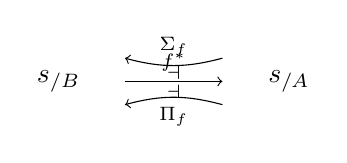
\begin{tikzpicture}[x=1.6em,y=1.5em]
  \node (lb) at (0,0)   {$s\Set_{/B}$};
  \node (rb) at (5.2,0) {$s\Set_{/A}$};
  \draw[->] (3.7,0.56) to[bend left=15] node[above,pos=0.5]{$\scriptstyle\Sigma_{f}$} (1.5,0.56);
  \node at (2.6,0.22) {$\scriptstyle\dashv$};
  \draw[->] (1.5,0) -- node[above]{$\scriptstyle f^{*}$} (3.7,0);
  \node at (2.6,-0.26) {$\scriptstyle\dashv$};
  \draw[->] (3.7,-0.56) to[bend right=15] node[below,pos=0.5]{$\scriptstyle\Pi_{f}$} (1.5,-0.56);
\end{tikzpicture}
\end{rveq}

对诸\trQuasiCategory{}之间的某些——但非全部——\trIsofibration{}
$f\colon A\twoheadrightarrow B$，这些\trAdjunction{}限制为保持%
\trIsofibration{}的\trFunctor
\begin{center}
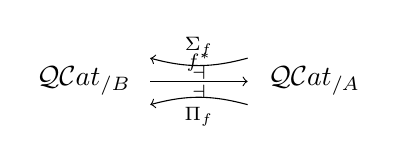
\begin{tikzpicture}[x=1.6em,y=1.5em]
  \node (lb) at (0,0)   {$\QCat_{/B}$};
  \node (rb) at (5.2,0) {$\QCat_{/A}$};
  \draw[->] (3.7,0.56) to[bend left=15] node[above,pos=0.5]{$\scriptstyle\Sigma_{f}$} (1.5,0.56);
  \node at (2.6,0.22) {$\scriptstyle\dashv$};
  \draw[->] (1.5,0) -- node[above]{$\scriptstyle f^{*}$} (3.7,0);
  \node at (2.6,-0.26) {$\scriptstyle\dashv$};
  \draw[->] (3.7,-0.56) to[bend right=15] node[below,pos=0.5]{$\scriptstyle\Pi_{f}$} (1.5,-0.56);
\end{tikzpicture}
\end{center}
此时 $f^{*}$ 与 $\Pi_{f}$ 都是宇宙论的。这样的\trIsofibration{}
$f\colon A\twoheadrightarrow B$ 称为\textbf{可指数化的}（exponentiable）。%
\footnote{一个著名的不可指数化\trFunctor{}出现于\cref{ex:nonexponentiable-d1}。}

由 Lurie 给出的、诸\trQuasiCategory{}之间可指数化\trFunctor{}的一个刻画——
他称之为「平坦纤维化」（flat fibrations）——出现于 [80, \S B.3]；一个模型
无关的刻画由 Ayala 与 Francis 给出于 [5, 2.2.8]。就我们此处的目的而言，我们
只需要：诸\trQuasiCategory{}之间的\trCocartesianFibration{}与%
\trCartesianFibration{}位列可指数化\trFunctor{}之中，而且二者分别保持%
\trCartesianFibration{}与\trCocartesianFibration。事实上，正如我们在 [114]
中所注意到的，由此得到的诸前推构造十分适配于宇宙论语境：

\begin{theorem}[{[114, 6.2.9--10]}]\label{thm:quasi-category-pushforward}
对诸\trQuasiCategory{}之间的一条\trCocartesianFibration{}
$q\colon E\twoheadrightarrow B$ 或\trCartesianFibration{}
$p\colon E\twoheadrightarrow B$，沿 $q$ 或 $p$ 的\trPullback{}容有一个右伴随，
该右伴随限制到诸宇宙论嵌入的∞-宇宙
\begin{center}
\begin{tikzpicture}[x=1.7em,y=1.6em]
  \node (qe) at (0,1.6)  {$\QCat_{/E}$};
  \node (qb) at (4.6,1.6){$\QCat_{/B}$};
  \draw[->] (3.4,2.18) to[bend left=15] node[above,pos=0.5]{$\scriptstyle q^{*}$} (1.2,2.18);
  \node at (2.3,1.82) {$\scriptstyle\dashv$};
  \draw[->] (1.2,1.02) to[bend right=15] node[below,pos=0.5]{$\scriptstyle\Pi_{q}$} (3.4,1.02);
  \node (ce) at (0,0)  {$\Cart(\QCat)_{/E}$};
  \node (cb) at (4.6,0){$\Cart(\QCat)_{/B}$};
  \draw[->] (3.3,0.44) to[bend left=15] node[above,pos=0.5]{$\scriptstyle q^{*}$} (1.3,0.44);
  \node at (2.3,0.1) {$\scriptstyle\dashv$};
  \draw[->] (1.3,-0.42) to[bend right=15] node[below,pos=0.5]{$\scriptstyle\Pi_{q}$} (3.3,-0.42);
  \draw[right hook->] (0,0.5) -- (0,1.08);
  \draw[right hook->] (4.6,0.5) -- (4.6,1.08);
  \begin{scope}[shift={(10.4,0)}]
    \node (pe) at (0,1.6)  {$\QCat_{/E}$};
    \node (pb) at (4.6,1.6){$\QCat_{/B}$};
    \draw[->] (3.4,2.18) to[bend left=15] node[above,pos=0.5]{$\scriptstyle p^{*}$} (1.2,2.18);
    \node at (2.3,1.82) {$\scriptstyle\dashv$};
    \draw[->] (1.2,1.02) to[bend right=15] node[below,pos=0.5]{$\scriptstyle\Pi_{p}$} (3.4,1.02);
    \node (oce) at (0,0)  {$\coCart(\QCat)_{/E}$};
    \node (ocb) at (4.6,0){$\coCart(\QCat)_{/B}$};
    \draw[->] (3.3,0.44) to[bend left=15] node[above,pos=0.5]{$\scriptstyle p^{*}$} (1.3,0.44);
    \node at (2.3,0.1) {$\scriptstyle\dashv$};
    \draw[->] (1.3,-0.42) to[bend right=15] node[below,pos=0.5]{$\scriptstyle\Pi_{p}$} (3.3,-0.42);
    \draw[right hook->] (0,0.5) -- (0,1.08);
    \draw[right hook->] (4.6,0.5) -- (4.6,1.08);
  \end{scope}
\end{tikzpicture}
\end{center}
之上，而且所有这些\trFunctor{}都是宇宙论的。
\end{theorem}

Lurie 关于\trCartesianFibration{}与\trCocartesianFibration{}可指数化的证明
可在 [80, B.3.11, B.4.5] 中找到；另见 [78, 3.2.2.12] 与 [80, B.4.2]。把这些
结果特例化到一个与此处所论情形远为接近的语境中，即 [115, 2.24]。

现在，我们把这些结果扩张到任意的 $(\infty,1)$-\trCategory{}的%
\trInfinityCosmos。

\begin{theorem}\label{thm:cosmos-pushforward}
对 $(\infty,1)$-\trCategory{}的\trInfinityCosmos{} $\mathcal{K}$ 中的一条%
\trCocartesianFibration{} $q\colon E\twoheadrightarrow B$ 或%
\trCartesianFibration{} $p\colon E\twoheadrightarrow B$，沿 $q$ 或 $p$ 的%
\trPullback{}容有一个拟伪函子性的右双伴随，该右双伴随限制到诸宇宙论嵌入的
∞-宇宙
\begin{center}
\begin{tikzpicture}[x=1.7em,y=1.6em]
  \node (ke) at (0,1.6)  {$\mathcal{K}_{/E}$};
  \node (kb) at (4.6,1.6){$\mathcal{K}_{/B}$};
  \draw[->] (3.4,2.18) -- ++(-0.36,0.07) -- ++(-0.36,-0.14) -- ++(-0.36,0.14)
    -- ++(-0.36,-0.14) -- ++(-0.36,0.14) -- ++(-0.36,-0.14) -- ++(-0.37,0.07);
  \node at (2.3,2.5) {$\scriptstyle q^{*}$};
  \node at (2.3,1.82) {$\scriptstyle\dashv$};
  \draw[->] (1.2,1.02) -- ++(0.36,-0.07) -- ++(0.36,0.14) -- ++(0.36,-0.14)
    -- ++(0.36,0.14) -- ++(0.36,-0.14) -- ++(0.36,0.14) -- ++(0.37,-0.07);
  \node at (2.3,0.68) {$\scriptstyle\Pi_{q}$};
  \node (ce) at (0,0)  {$\Cart(\mathcal{K})_{/E}$};
  \node (cb) at (4.6,0){$\Cart(\mathcal{K})_{/B}$};
  \draw[->] (3.3,0.44) -- ++(-0.33,0.07) -- ++(-0.33,-0.14) -- ++(-0.33,0.14)
    -- ++(-0.33,-0.14) -- ++(-0.33,0.14) -- ++(-0.34,0.07);
  \node at (2.3,0.72) {$\scriptstyle q^{*}$};
  \node at (2.3,0.1) {$\scriptstyle\dashv$};
  \draw[->] (1.3,-0.42) -- ++(0.33,-0.07) -- ++(0.33,0.14) -- ++(0.33,-0.14)
    -- ++(0.33,0.14) -- ++(0.33,-0.14) -- ++(0.34,0.07);
  \node at (2.3,-0.72) {$\scriptstyle\Pi_{q}$};
  \draw[right hook->] (0,0.5) -- (0,1.08);
  \draw[right hook->] (4.6,0.5) -- (4.6,1.08);
  \begin{scope}[shift={(10.4,0)}]
    \node (pe) at (0,1.6)  {$\mathcal{K}_{/E}$};
    \node (pb) at (4.6,1.6){$\mathcal{K}_{/B}$};
    \draw[->] (3.4,2.18) -- ++(-0.36,0.07) -- ++(-0.36,-0.14) -- ++(-0.36,0.14)
      -- ++(-0.36,-0.14) -- ++(-0.36,0.14) -- ++(-0.36,-0.14) -- ++(-0.37,0.07);
    \node at (2.3,2.5) {$\scriptstyle p^{*}$};
    \node at (2.3,1.82) {$\scriptstyle\dashv$};
    \draw[->] (1.2,1.02) -- ++(0.36,-0.07) -- ++(0.36,0.14) -- ++(0.36,-0.14)
      -- ++(0.36,0.14) -- ++(0.36,-0.14) -- ++(0.36,0.14) -- ++(0.37,-0.07);
    \node at (2.3,0.68) {$\scriptstyle\Pi_{p}$};
    \node (oce) at (0,0)  {$\coCart(\mathcal{K})_{/E}$};
    \node (ocb) at (4.6,0){$\coCart(\mathcal{K})_{/B}$};
    \draw[->] (3.3,0.44) -- ++(-0.33,0.07) -- ++(-0.33,-0.14) -- ++(-0.33,0.14)
      -- ++(-0.33,-0.14) -- ++(-0.33,0.14) -- ++(-0.34,0.07);
    \node at (2.3,0.72) {$\scriptstyle p^{*}$};
    \node at (2.3,0.1) {$\scriptstyle\dashv$};
    \draw[->] (1.3,-0.42) -- ++(0.33,-0.07) -- ++(0.33,0.14) -- ++(0.33,-0.14)
      -- ++(0.33,0.14) -- ++(0.33,-0.14) -- ++(0.34,0.07);
    \node at (2.3,-0.72) {$\scriptstyle\Pi_{p}$};
    \draw[right hook->] (0,0.5) -- (0,1.08);
    \draw[right hook->] (4.6,0.5) -- (4.6,1.08);
  \end{scope}
\end{tikzpicture}
\end{center}
之上，

而陈述中的「双伴随性」——再次挪用弱 2-范畴论的一个术语——意指一个拟伪自然
的\trEquivalence：
\begin{center}
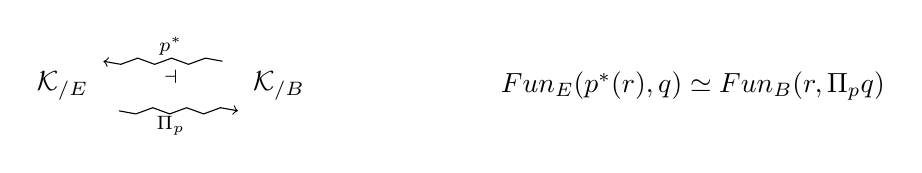
\begin{tikzpicture}[x=1.7em,y=1.6em]
  \node (ke) at (0,0)  {$\mathcal{K}_{/E}$};
  \node (kb) at (4.6,0){$\mathcal{K}_{/B}$};
  \draw[->] (3.4,0.56) -- ++(-0.36,0.07) -- ++(-0.36,-0.14) -- ++(-0.36,0.14)
    -- ++(-0.36,-0.14) -- ++(-0.36,0.14) -- ++(-0.36,-0.14) -- ++(-0.37,0.07);
  \node at (2.3,0.9) {$\scriptstyle p^{*}$};
  \node at (2.3,0.22) {$\scriptstyle\dashv$};
  \draw[->] (1.2,-0.56) -- ++(0.36,-0.07) -- ++(0.36,0.14) -- ++(0.36,-0.14)
    -- ++(0.36,0.14) -- ++(0.36,-0.14) -- ++(0.36,0.14) -- ++(0.37,-0.07);
  \node at (2.3,-0.9) {$\scriptstyle\Pi_{p}$};
  \node at (13.4,0) {$\Fun_{E}(p^{*}(r),q)\simeq\Fun_{B}(r,\Pi_{p}q)$};
\end{tikzpicture}
\end{center}
\end{theorem}

\begin{proof}
对一条余/笛卡尔纤维化 $p\colon E\twoheadrightarrow B$，前推拟伪函子
$\Pi_{p}\colon\mathcal{K}_{/E}\rightsquigarrow\mathcal{K}_{/B}$ 定义为：与
介于诸\trQuasiCategory{}之间的底余/笛卡尔纤维化
$p_{0}\colon E_{0}\to B_{0}$ 相关联的前推，与宇宙论双等价的之字形链

\begin{rveq}\label{eq:pushforward-slice-zigzag}
\begin{tikzpicture}[x=1.6em,y=1.5em]
  \node (ke)  at (0,1.5)   {$\mathcal{K}_{/E}$};
  \node (kb)  at (4.6,1.5) {$\mathcal{K}_{/B}$};
  \draw[->] (1.1,1.5) -- ++(0.42,0.07) -- ++(0.42,-0.14) -- ++(0.42,0.14)
    -- ++(0.42,-0.14) -- ++(0.42,0.14) -- ++(0.42,-0.14) -- ++(0.43,0.07);
  \node at (2.85,1.92) {$\scriptstyle\Pi_{p}$};
  \draw[->] (0,1.0) -- node[left]{$\scriptstyle(-)_{0}$} (0,0.5);
  \node at (2.3,0.78) {$\scriptstyle\simeq$};
  \draw[right hook->] (4.6,1.0) -- node[right]{$\scriptstyle(-)_{0}$} (4.6,0.5);
  \node (qe) at (0,0)   {$\QCat_{/E_{0}}$};
  \node (qb) at (4.6,0) {$\QCat_{/B_{0}}$};
  \draw[->] (1.1,0) -- node[below]{$\scriptstyle\Pi_{p_{0}}$} (3.5,0);
\end{tikzpicture}
\end{rveq}
给出的。注意：\trPullback{}与前推二者都与切片化的底拟范畴\trFunctor{}
$(-)_{0}\colon\mathcal{K}_{/B}\Rightarrow\QCat_{/B_{0}}$ 在等价的意义下
交换。

依据下列复合\trEquivalence，这个复合拟伪函子可以理解为一个逐点的右双伴随
\[
\begin{gathered}
\Fun_{E}(p^{*}(r),q)\xrightarrow{\;(-)_{0}\;}\Fun_{E_{0}}((p_{0})^{*}(r_{0}),q_{0})\\
\parallel\\
\Fun_{B_{0}}(r_{0},\Pi_{p_{0}}(q_{0}))\xleftarrow{\;(-)_{0}\;}\Fun_{B}(r,\Pi_{p}q)
\end{gathered}
\]
它们在 $q\colon F\twoheadrightarrow E$ 与 $r\colon G\twoheadrightarrow B$ 中
是拟伪自然地定义的。这就证明了第一款陈述。

现在，设 $p\colon E\twoheadrightarrow B$ 是 $\mathcal{K}$ 中的一条%
\trCartesianFibration，并设 $q\colon F\twoheadrightarrow E$ 是一条%
\trCocartesianFibration。那么由第 10 章中的命题 10.3.6，$\Pi_{p}q$ 是
$\mathcal{K}$ 中的\trCocartesianFibration，当且仅当其底\trFunctor{}是诸%
\trQuasiCategory{}上的\trCocartesianFibration。由 \eqref{eq:pushforward-slice-zigzag}
的本质交换性，这个\trFunctor{}等价于 $\Pi_{p_{0}}(q_{0})$，而由%
\cref{thm:quasi-category-pushforward}，后者是诸\trQuasiCategory{}的一条%
\trCocartesianFibration。由于余笛卡尔纤维化性在等价之下是重满的，保持结果
随之而来。前推保持笛卡尔函子的证明类似地成立。

最后，\cref{thm:quasi-category-pushforward}证明：诸\trQuasiCategory{}的余笛卡尔
纤维化之间的\trCartesianFunctor{}在 $p^{*}\dashv\Pi_{p}$ 之下转置为笛卡尔
函子。由于\trCartesianFunctor{}被诸宇宙论双等价保持并反射，同样的事情在任何
$(\infty,1)$-\trCategory{}的\trInfinityCosmos{}中成立。于是，拟伪自然的%
\trEquivalence{} $\Fun_{E}(p^{*}(r),q)\simeq\Fun_{B}(r,\Pi_{p}q)$ 限制而定义
一个拟伪自然的\trEquivalence{}
$\Fun^{\mathit{cart}}_{E}(p^{*}(r),q)\simeq\Fun^{\mathit{cart}}_{B}(r,\Pi_{p}q)$。
\end{proof}


\begin{lemma}[Beck--Chevalley]\label{lem:beck-chevalley-qcat}
考虑 $(\infty,1)$-\trCategory{}的\trInfinityCosmos{}中的一个\trPullback{}图
\begin{center}
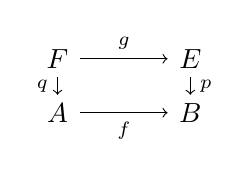
\begin{tikzpicture}[x=1.5em,y=1.3em]
  \node (f) at (0,1.5) {$F$};
  \node (e) at (3.2,1.5) {$E$};
  \node (a) at (0,0)   {$A$};
  \node (b) at (3.2,0) {$B$};
  \draw[->] (0.55,1.5) -- node[above]{$\scriptstyle g$} (2.65,1.5);
  \draw[->] (0,1.0) -- node[left]{$\scriptstyle q$} (0,0.5);
  \draw[->] (3.2,1.0) -- node[right]{$\scriptstyle p$} (3.2,0.5);
  \draw[->] (0.55,0) -- node[below]{$\scriptstyle f$} (2.65,0);
  \node at (0.62,0.95) {$\scriptstyle\lrcorner$};
\end{tikzpicture}
\end{center}
并设 $p$ 是一条\trCocartesianFibration{}或\trCartesianFibration。那么对一切
$r\colon G\twoheadrightarrow E$，诸映射
$f^{*}\Pi_{p}r\simeq\Pi_{q}g^{*}r$ 在 $A$ 之上等价。
\end{lemma}

\begin{proof}
施用宇宙论双等价 $(-)_{0}\colon\mathcal{K}\Rightarrow\QCat$，只需对诸%
\trQuasiCategory{}证明本引理；此时所论的诸\trFunctor{}容有左伴随：
\begin{center}
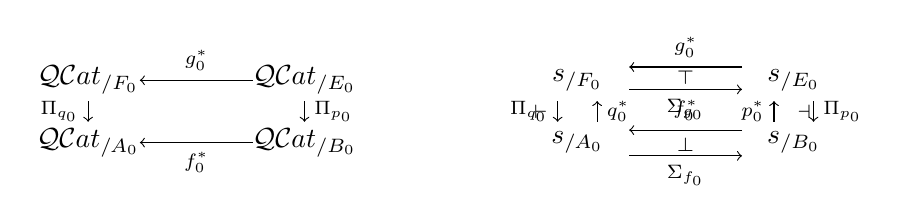
\begin{tikzpicture}[x=1.7em,y=1.5em]
  \node (a) at (0,1.5)  {$\QCat_{/F_{0}}$};
  \node (b) at (4.6,1.5){$\QCat_{/E_{0}}$};
  \draw[->] (3.5,1.5) -- node[above]{$\scriptstyle g_{0}^{*}$} (1.1,1.5);
  \draw[->] (0,1.0) -- node[left]{$\scriptstyle\Pi_{q_{0}}$} (0,0.5);
  \draw[->] (4.6,1.0) -- node[right]{$\scriptstyle\Pi_{p_{0}}$} (4.6,0.5);
  \node (c) at (0,0)  {$\QCat_{/A_{0}}$};
  \node (d) at (4.6,0){$\QCat_{/B_{0}}$};
  \draw[->] (3.5,0) -- node[below]{$\scriptstyle f_{0}^{*}$} (1.1,0);
  \begin{scope}[shift={(10.4,0)}]
    \node (a2) at (0,1.5)  {$s\Set_{/F_{0}}$};
    \node (b2) at (4.6,1.5){$s\Set_{/E_{0}}$};
    \draw[->] (3.5,1.82) -- node[above]{$\scriptstyle g_{0}^{*}$} (1.1,1.82);
    \node at (2.3,1.56) {$\scriptstyle\top$};
    \draw[->] (1.1,1.28) -- node[below]{$\scriptstyle\Sigma_{g_{0}}$} (3.5,1.28);
    \draw[->] (-0.42,1.0) -- node[left]{$\scriptstyle\Pi_{q_{0}}$} (-0.42,0.5);
    \node at (-0.78,0.75) {$\scriptstyle\vdash$};
    \draw[->] (0.42,0.5) -- node[right]{$\scriptstyle q_{0}^{*}$} (0.42,1.0);
    \draw[->] (4.18,0.5) -- node[left]{$\scriptstyle p_{0}^{*}$} (4.18,1.0);
    \node at (4.82,0.75) {$\scriptstyle\dashv$};
    \draw[->] (5.02,1.0) -- node[right]{$\scriptstyle\Pi_{p_{0}}$} (5.02,0.5);
    \node (c2) at (0,0)  {$s\Set_{/A_{0}}$};
    \node (d2) at (4.6,0){$s\Set_{/B_{0}}$};
    \draw[->] (1.1,-0.32) -- node[below]{$\scriptstyle\Sigma_{f_{0}}$} (3.5,-0.32);
    \node at (2.3,-0.06) {$\scriptstyle\perp$};
    \draw[->] (3.5,0.3) -- node[above]{$\scriptstyle f_{0}^{*}$} (1.1,0.3);
  \end{scope}
\end{tikzpicture}
\end{center}

对单纯集之间的任何映射 $a\colon X\to A_{0}$，通过检视如下\trPullback{}矩形
\begin{center}
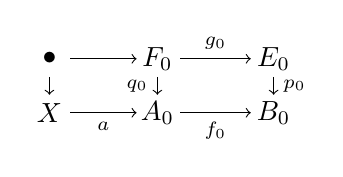
\begin{tikzpicture}[x=1.5em,y=1.3em]
  \node (x1) at (0,1.5)  {$\bullet$};
  \node (f0) at (2.6,1.5){$F_{0}$};
  \node (e0) at (5.4,1.5){$E_{0}$};
  \node (x2) at (0,0)    {$X$};
  \node (a0) at (2.6,0)  {$A_{0}$};
  \node (b0) at (5.4,0)  {$B_{0}$};
  \draw[->] (0.5,1.5) -- (2.1,1.5);
  \draw[->] (3.15,1.5) -- node[above]{$\scriptstyle g_{0}$} (4.85,1.5);
  \draw[->] (0,1.0) -- (0,0.5);
  \draw[->] (2.6,1.0) -- node[left]{$\scriptstyle q_{0}$} (2.6,0.5);
  \draw[->] (5.4,1.0) -- node[right]{$\scriptstyle p_{0}$} (5.4,0.5);
  \draw[->] (0.5,0) -- node[below]{$\scriptstyle a$} (2.1,0);
  \draw[->] (3.15,0) -- node[below]{$\scriptstyle f_{0}$} (4.85,0);
  \node at (2.05,0.98) {$\scriptstyle\lrcorner$};
  \node at (3.18,0.98) {$\scriptstyle\lrcorner$};
\end{tikzpicture}
\end{center}
显然有 $\Sigma_{g_{0}}q_{0}^{*}a\cong p_{0}^{*}\Sigma_{f_{0}}a$。于是，右伴随
$f_{0}^{*}\Pi_{p_{0}}\cong\Pi_{q_{0}}g_{0}^{*}$ 也在\trIsomorphism{}的意义下
交换，而保守性给出 $\mathcal{K}$ 中所宣称的\trEquivalence。
\end{proof}

现在我们来解释我们对这些结果的兴趣所在。由第 9 章中的%
\cref{def:right-extension-lifting-modules}回忆起：模 $A\xrightarrow{G}C$ 沿模
$A\xrightarrow{E}B$ 的一个\textbf{右扩张}，由一个数对给出——其中一支模
$B\xrightarrow{\hom_{A}(E,G)}C$ 连同一支二元\trCell
\begin{center}
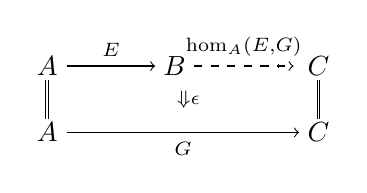
\begin{tikzpicture}[x=1em,y=1em]
  \node at (0,1.2)    {$A$};
  \node at (4.6,1.2)  {$B$};
  \node at (9.8,1.2)  {$C$};
  \node at (0,-1.2)   {$A$};
  \node at (9.8,-1.2) {$C$};
  \draw[->] (0.7,1.2)  -- node[above]{$\scriptstyle E$} (3.9,1.2);
  \draw[->,dashed] (5.3,1.2) -- node[above]{$\scriptstyle\hom_{A}(E,G)$} (8.9,1.2);
  \draw (8.35,1.12) -- (8.35,1.28);
  \draw[->] (0.7,-1.2) -- node[below]{$\scriptstyle G$} (9.1,-1.2);
  \draw[double,double distance=0.6pt] (0,0.7)   -- (0,-0.7);
  \draw[double,double distance=0.6pt] (9.8,0.7) -- (9.8,-0.7);
  \node at (5.1,0) {$\scriptstyle\Downarrow\epsilon$};
\end{tikzpicture}
\end{center}
构成，该\trCell{}在模的\trVirtualEquipment{}中的诸\trCell{}之间按彼处详述的
意义是泛的。对偶地，$A\xrightarrow{G}C$ 穿过 $B\xrightarrow{F}C$ 的一个%
\textbf{右提升}，由一个数对给出——其中一支模
$A\xrightarrow{\hom(F,G)_{C}}B$ 连同一支泛的二元\trCell
\begin{center}
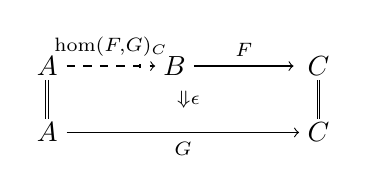
\begin{tikzpicture}[x=1em,y=1em]
  \node at (0,1.2)    {$A$};
  \node at (4.6,1.2)  {$B$};
  \node at (9.8,1.2)  {$C$};
  \node at (0,-1.2)   {$A$};
  \node at (9.8,-1.2) {$C$};
  \draw[->,dashed] (0.7,1.2) -- node[above]{$\scriptstyle\hom(F,G)_{C}$} (3.9,1.2);
  \draw (3.35,1.12) -- (3.35,1.28);
  \draw[->] (5.3,1.2)  -- node[above]{$\scriptstyle F$} (8.9,1.2);
  \draw[->] (0.7,-1.2) -- node[below]{$\scriptstyle G$} (9.1,-1.2);
  \draw[double,double distance=0.6pt] (0,0.7)   -- (0,-0.7);
  \draw[double,double distance=0.6pt] (9.8,0.7) -- (9.8,-0.7);
  \node at (5.1,0) {$\scriptstyle\Downarrow\epsilon$};
\end{tikzpicture}
\end{center}
构成。此处我们为这些概念引入不同的记号，意在给它们改换名目。我们把模
$\hom_{A}(E,G)$ 称为从 $E$ 到 $G$ 的\textbf{左 hom}（left hom）\footnote{原书
此处行文作「the left hom from $E$ to $F$」，且 p.489 右扩张展示图之第二模标签
亦印作 $\hom_{A}(E,F)$；按本条首句（结果模为 $\hom_{A}(E,G)$）与下句
「homomorphisms from $E$ to $G$」，两处 $F$ 均系 $G$ 之误，径改。——译者注}，把
$\hom(F,G)_{C}$ 称为从 $F$ 到 $G$ 的\textbf{右 hom}（right hom）。延伸
「模」这一隐喻，我们把左 hom 设想为从 $E$ 到 $G$ 的、尊重左 $A$-作用的诸%
\trHomomorphism{}之对象，而右 hom 则是从 $F$ 到 $G$ 的、尊重右 $C$-作用的诸\trHomomorphism{}之对象。
我们本节的第一个目标，是论证诸\trQuasiCategory{}之间的模的%
\trVirtualEquipment{}对一切合适的模对都拥有左 hom 与右 hom。由%
\trModelIndependence，这一结果扩张到任何 $(\infty,1)$-\trCategory{}的%
\trInfinityCosmos。

\begin{theorem}\label{thm:module-equipment-biclosed}
诸\trQuasiCategory{}之间的模的\trVirtualEquipment{}是\textbf{双闭的}
（biclosed），容有满足一个富集\trUniversalProperty{}的左 hom 与右 hom：对模
$A\xrightarrow{E}B$、$B\xrightarrow{F}C$ 与 $A\xrightarrow{G}C$，
\[
\Fun_{A\times B}\bigl(E,\hom(F,G)_{C}\bigr)\cong
\Fun_{A\times C}(E\times_{B}F,G)\cong
\Fun_{B\times C}\bigl(F,\hom_{A}(E,G)\bigr).
\]
\end{theorem}

\begin{proof}
左 hom 与右 hom 的情形是对偶的，故我们聚焦于前者。固定一条模
$A\overset{q}{\twoheadleftarrow}E\overset{p}{\twoheadrightarrow}B$，把
$\hom_{A}(E,G)$ 定义为模 $A\xrightarrow{G}C$ 在下列复合右伴随\trFunctor{}%
之下的像：
\begin{center}
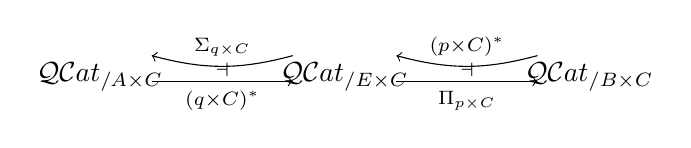
\begin{tikzpicture}[x=1.7em,y=1.5em]
  \node (a) at (0,0)    {$\QCat_{/A\times C}$};
  \node (b) at (5.2,0)  {$\QCat_{/E\times C}$};
  \node (c) at (10.4,0) {$\QCat_{/B\times C}$};
  \draw[->] (4.1,0.52) to[bend left=15] node[above,pos=0.5]{$\scriptstyle\Sigma_{q\times C}$} (1.1,0.52);
  \node at (2.6,0.18) {$\scriptstyle\dashv$};
  \draw[->] (1.1,-0.1) -- node[below]{$\scriptstyle(q\times C)^{*}$} (4.1,-0.1);
  \draw[->] (9.3,0.52) to[bend left=15] node[above,pos=0.5]{$\scriptstyle(p\times C)^{*}$} (6.3,0.52);
  \node at (7.8,0.18) {$\scriptstyle\dashv$};
  \draw[->] (6.3,-0.1) -- node[below]{$\scriptstyle\Pi_{p\times C}$} (9.3,-0.1);
\end{tikzpicture}
\end{center}
注意：该左伴随把双侧等价纤维化
$B\overset{s}{\twoheadleftarrow}F\overset{r}{\twoheadrightarrow}C$ 带为复合
双侧等价纤维化
\begin{center}
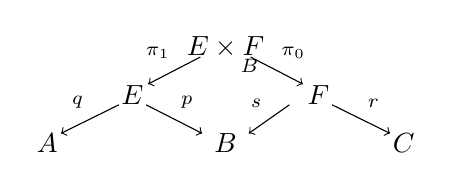
\begin{tikzpicture}[x=1.4em,y=1.15em]
  \node (ef) at (0,3.0)  {$E\times F$};
  \node at (0.62,2.42)   {$\scriptstyle B$};
  \node (e)  at (-2.4,1.5){$E$};
  \node (f)  at (2.4,1.5) {$F$};
  \node (a)  at (-4.6,0)  {$A$};
  \node (b)  at (0,0)     {$B$};
  \node (c)  at (4.6,0)   {$C$};
  \draw[->] (-0.65,2.7) -- node[above left,pos=0.4]{$\scriptstyle\pi_{1}$} (-2.0,1.85);
  \draw[->] (0.65,2.7)  -- node[above right,pos=0.4]{$\scriptstyle\pi_{0}$} (2.0,1.85);
  \node at (0.35,2.2) {$\scriptstyle\lrcorner$};
  \draw[->] (-2.75,1.2) -- node[above left,pos=0.45]{$\scriptstyle q$} (-4.25,0.3);
  \draw[->] (-2.05,1.2) -- node[above right,pos=0.45]{$\scriptstyle p$} (-0.6,0.3);
  \draw[->] (1.65,1.2)  -- node[above left,pos=0.45]{$\scriptstyle s$} (0.6,0.3);
  \draw[->] (2.75,1.2)  -- node[above right,pos=0.45]{$\scriptstyle r$} (4.25,0.3);
\end{tikzpicture}
\end{center}
而单纯富集的伴随性给出诸\trQuasiCategory{}之间的自然等价（在此情形中即%
\trIsomorphism）
\[
\Fun_{A\times C}(E\times_{B}F,G)\cong
\Fun_{B\times C}\bigl(F,\hom_{A}(E,G)\bigr).
\]

这些\trEquivalence{}在这些\trQuasiCategory{}的对象的同构类之集合上诱导双射。
由第 8 章中的命题 8.1.6，这就给出了右 hom 在模的\trVirtualEquipment{}中所需
的\trUniversalProperty（见\cref{ex:module-cell-right-extension}）——至少一旦我们证明了：当 $E$ 与 $G$
是模时，$\hom_{A}(E,G)$ 定义一条模。

于是，尚待证明的只是：当 $A\xrightarrow{E}B$
是一条模时，\trFunctor
\[
\hom_{A}(E,-)\colon\QCat_{/A\times C}
  \xrightarrow{\;(q\times C)^{*}\;}\QCat_{/E\times C}
  \xrightarrow{\;\Pi_{p\times C}\;}\QCat_{/B\times C}
\]
保持模。

第 7 章中的命题 7.4.5 告诉我们：模在\trPullback{}之下稳定，故我们只需论证：
$\Pi_{p\times C}$ 把一条模
$E\overset{v}{\twoheadleftarrow}M\overset{u}{\twoheadrightarrow}C$ 带为一条
从 $B$ 到 $C$ 的模。第 7 章中的命题 7.4.2 把从 $E$ 到 $C$ 的模刻画为那些满足
如下条件的双侧等价纤维化 $(v,u)\colon M\twoheadrightarrow E\times C$：
\begin{enumerate}[label=(\roman*)]
\item $(v,u)\colon M\twoheadrightarrow E\times C$ 是 $\QCat_{/C}$ 中的一条%
  \trCocartesianFibration，
\item $(v,u)\colon M\twoheadrightarrow E\times C$ 是 $\QCat_{/E}$ 中的一条%
  \trCartesianFibration，
\item $(v,u)\colon M\twoheadrightarrow E\times C$ 作为 $\QCat_{/E\times C}$
  中的对象是\trDiscrete。
\end{enumerate}
我们将证明 $\Pi_{p\times C}$ 保持这些性质中的每一条，从而断定 $\Pi_{p\times C}M$
定义一条从 $B$ 到 $C$ 的模。(iii) 的保持是自动的：\cref{thm:quasi-category-pushforward}
表明前推是一个宇宙论\trFunctor，而第 1 章中的%
\cref{rem:cosmological-discrete-categories}观察到宇宙论\trFunctor{}保持%
\trDiscrete{}对象。

为证 (ii)，我们必须证明 $\Pi_{p\times C}M\twoheadrightarrow B\times C$ 是
$\QCat_{/B}$ 中的一条\trCartesianFibration。首先，由第 10 章中的命题 10.1.4
注意到：宇宙论\trFunctor{} $\Pi_{p}\colon\QCat_{/E}\to\QCat_{/B}$ 保持%
\trCartesianFibration，\footnote{这并非\cref{thm:cosmos-pushforward}的一个
应用——在该语境中，\cref{thm:cosmos-pushforward}会告诉我们 $\Pi_{p}$ 把
$E$ 之上的一条\trCocartesianFibration{}带到 $B$ 之上的一条%
\trCocartesianFibration。不如说，我们注意到：$\Pi_{p}$ 仅凭其为宇宙论的这
一点，就把介于余定义域为 $E$ 的诸\trIsofibration{}之间的%
\trCartesianFibration，带为介于余定义域为 $B$ 的诸\trIsofibration{}之间的%
\trCartesianFibration。}于是我们断定 $\Pi_{p}M\twoheadrightarrow\Pi_{p}(B\times C)$
是 $\QCat_{/B}$ 中的一条\trCartesianFibration。然而，这个\trFunctor{}与
$\Pi_{p\times C}M\twoheadrightarrow B\times C$ 并不重合。不如说，正如下面的
\cref{lem:pushforward-image-pullback}所证明的，$\Pi_{p\times C}M\twoheadrightarrow B\times C$
是 $\Pi_{p}M\twoheadrightarrow\Pi_{p}(B\times C)$ 在 $\QCat_{/B}$ 中的一个%
\trPullback，故由\trCartesianFibration{}的拉回稳定性，这就证明了 (ii)。

为证余下的性质 (i)，由第 7 章中的\cref{lem:cartesian-on-the-right}回忆起：
说 $(v,u)\colon M\twoheadrightarrow E\times C$ 定义 $\QCat_{/C}$ 中的一条%
\trCocartesianFibration，等价于说 $(v,u)\colon M\twoheadrightarrow E\times C$
在子∞-宇宙 $\coCart(\QCat)_{/E}\subset\QCat_{/E}$ 中定义一个态射。由%
\cref{thm:quasi-category-pushforward}，前推限制而定义一个宇宙论\trFunctor{}
$\Pi_{p}\colon\coCart(\QCat)_{/E}\to\coCart(\QCat)_{/B}$，故
$\Pi_{p}M\twoheadrightarrow\Pi_{p}(E\times C)$ 居于子宇宙
$\coCart(\QCat)_{/B}\subset\QCat_{/B}$ 之中。由于\trPullback{}由宇宙论嵌入
$\coCart(\QCat)_{/B}\hookrightarrow\QCat_{/B}$ 所创造，由%
\cref{lem:pushforward-image-pullback}，$\Pi_{p\times C}M\twoheadrightarrow B\times C$
也居于子宇宙 $\coCart(\QCat)_{/B}\subset\QCat_{/B}$ 之中。于是，第 7 章中的%
\cref{lem:cartesian-on-the-right}告诉我们：$\Pi_{p\times C}M\twoheadrightarrow B\times C$
是 $\QCat_{/C}$ 中的一条\trCocartesianFibration，如所需。
\end{proof}

\begin{lemma}\label{lem:pushforward-image-pullback}
设 $p\colon E\twoheadrightarrow B$ 是诸\trQuasiCategory{}之间的一条%
\trCartesianFibration{}或\trCocartesianFibration。那么，一条\trIsofibration{}
$M\twoheadrightarrow E\times C$ 在
$\Pi_{p\times C}\colon\QCat_{/E\times C}\to\QCat_{/B\times C}$ 之下的像，就是
由如下\trPullback
\begin{center}
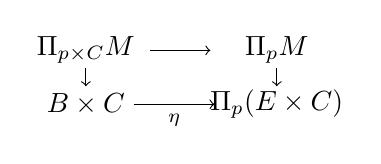
\begin{tikzpicture}[x=1.5em,y=1.3em]
  \node (tl) at (0,1.5)  {$\Pi_{p\times C}M$};
  \node (tr) at (4.6,1.5){$\Pi_{p}M$};
  \node (bl) at (0,0)    {$B\times C$};
  \node (br) at (4.6,0)  {$\Pi_{p}(E\times C)$};
  \draw[->] (1.55,1.5) -- (3.0,1.5);
  \draw[->] (0,1.0) -- (0,0.5);
  \draw[->] (4.6,1.0) -- (4.6,0.5);
  \draw[->] (1.15,0) -- node[below]{$\scriptstyle\eta$} (3.1,0);
  \node at (0.62,0.95) {$\scriptstyle\lrcorner$};
\end{tikzpicture}
\end{center}
所定义的左侧竖直\trIsofibration，其中右侧的竖直态射是映射
$M\twoheadrightarrow E\times C$ 在
$\Pi_{p}\colon\QCat_{/E}\to\QCat_{/B}$ 之下的像。
\end{lemma}

引理 12.3.7 的结论在等价意义下对任何 $(\infty,1)$-\trCategory{}的%
\trInfinityCosmos{} $\mathcal{K}$ 都成立（见\cref{ex:model-independent-lemma-12-3-7}）。然而我们发现，
与\cref{thm:cosmos-pushforward}的较弱伴随打交道，不如与%
\cref{thm:quasi-category-pushforward}的严格伴随打交道来得容易。

\begin{proof}
为使陈述有意义，注意到 $p^{*}$ 把 $\pi\colon B\times C\twoheadrightarrow B$
带为 $\pi\colon E\times C\twoheadrightarrow E$。于是，映射
$\eta\colon B\times C\to\Pi_{p}(E\times C)$ 是\trAdjunction{}
$p^{*}\dashv\Pi_{p}$ 的\trUnit{}的一个分量。现在，通过验证所示\trPullback{}%
具有定义 $\Pi_{p\times C}M\in\QCat_{/B\times C}$ 的那个\trUniversalProperty，
断言便直接得出。\trPullback{}图上的一个\trCone{}可以解读为 $\QCat_{/B}$ 中的
一个\trDiagram
\begin{center}
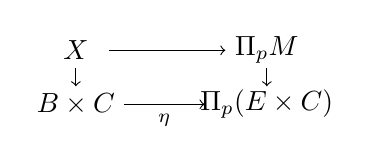
\begin{tikzpicture}[x=1.5em,y=1.3em]
  \node (tl) at (0,1.5) {$X$};
  \node (tr) at (4.6,1.5){$\Pi_{p}M$};
  \node (bl) at (0,0)   {$B\times C$};
  \node (br) at (4.6,0) {$\Pi_{p}(E\times C)$};
  \draw[->] (0.8,1.5) -- (3.6,1.5);
  \draw[->] (0,1.0) -- (0,0.5);
  \draw[->] (4.6,1.0) -- (4.6,0.5);
  \draw[->] (1.15,0) -- node[below]{$\scriptstyle\eta$} (3.1,0);
\end{tikzpicture}
\end{center}
后者转置而定义 $\QCat_{/E}$ 中的一个交换方块
\begin{center}
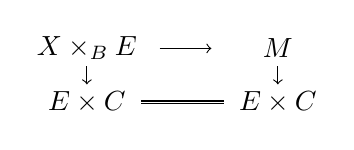
\begin{tikzpicture}[x=1.5em,y=1.3em]
  \node (tl) at (0,1.5) {$X\times_{B}E$};
  \node (tr) at (4.6,1.5){$M$};
  \node (bl) at (0,0)   {$E\times C$};
  \node (br) at (4.6,0) {$E\times C$};
  \draw[->] (1.75,1.5) -- (3.0,1.5);
  \draw[->] (0,1.0) -- (0,0.5);
  \draw[->] (4.6,1.0) -- (4.6,0.5);
  \draw[double,double distance=0.6pt] (1.3,0) -- (3.3,0);
\end{tikzpicture}
\end{center}
事实上，这个\trDiagram{}居于 $\QCat_{/E\times C}$ 之中，且左侧的竖直映射
$X\times_{B}E\twoheadrightarrow E\times C$ \trIsomorphism{}于
$(p\times C)^{*}(X\twoheadrightarrow B\times C)$。于是，这个方块沿
$(p\times C)^{*}\dashv\Pi_{p\times C}$ 转置为一个交换方块
\begin{center}
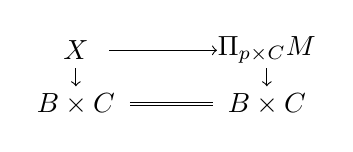
\begin{tikzpicture}[x=1.5em,y=1.3em]
  \node (tl) at (0,1.5) {$X$};
  \node (tr) at (4.6,1.5){$\Pi_{p\times C}M$};
  \node (bl) at (0,0)   {$B\times C$};
  \node (br) at (4.6,0) {$B\times C$};
  \draw[->] (0.8,1.5) -- (3.4,1.5);
  \draw[->] (0,1.0) -- (0,0.5);
  \draw[->] (4.6,1.0) -- (4.6,0.5);
  \draw[double,double distance=0.6pt] (1.3,0) -- (3.3,0);
\end{tikzpicture}
\end{center}
这就证明了断言。
\end{proof}

定理 12.3.6 的结果扩张到相互双等价的∞-宇宙：

\begin{corollary}\label{cor:module-equipment-biclosed-cosmos}
在一个 $(\infty,1)$-\trCategory{}的\trInfinityCosmos{}中，模的%
\trVirtualEquipment{}是双闭的，容有满足一个\emph{弱}富集\trUniversalProperty{}%
的左 hom 与右 hom：对模
$A\xrightarrow{E}B$、$B\xrightarrow{F}C$ 与 $A\xrightarrow{G}C$，
\[
\Fun_{A\times B}\bigl(E,\hom(F,G)_{C}\bigr)\simeq
\Fun_{A\times C}(E\times_{B}F,G)\simeq
\Fun_{B\times C}\bigl(F,\hom_{A}(E,G)\bigr).
\]
\end{corollary}

证明这个结果有两条策略。第一条是证明\cref{thm:module-equipment-biclosed}之
证明中所用诸配料的\trModelIndependence（见练习 12.3.iii）。一条更为便捷——
尽管归根结底信息量较少——的策略，是直接利用虚拟装备的双等价，这正是我们
此处采取的进路。

\begin{proof}
考虑 $(\infty,1)$-\trCategory{}的\trInfinityCosmos{}中的模
$A\xrightarrow{E}B$ 与 $A\xrightarrow{G}C$。由第 11 章中的%
\cref{thm:biequivalence-of-virtual-equipments}，存在一条模
$B\xrightarrow{R}C$，其\trUnderlyingQuasiCategory{}等价于%
\cref{thm:module-equipment-biclosed}的左 hom $\hom_{A_{0}}(E_{0},G_{0})$，
还存在一支二元\trCell{} $\nu\colon E\otimes R\Rightarrow G$，其在底
拟范畴\trFunctor{}之下的像与这个\trEquivalence{}复合，给出定义从 $E_{0}$ 到
$G_{0}$ 的左 hom 的那个介于诸\trQuasiCategory{}之间的模的二元映射。尚待
论证的只是：这份数据拥有 $\mathbb{M}od(\mathcal{K})$ 中右扩张的%
\trUniversalProperty，但这由虚拟装备的双等价
$(-)_{0}\colon\mathbb{M}od(\mathcal{K})\Rightarrow\mathbb{M}od(\QCat)$ 得出。
\end{proof}

左 hom 与右 hom 可用来定义那些在∞-\trCategory{}论中编码假想\trUniversalProperty{}%
的模。当如此构造的诸模视情形被一个\trFunctor{}协变地或反变地表示时，这份数据
便「满足泛性质」，我们现在来例示这一点。第 9 章中的\cref{prop:limits-from-slices}
观察到：\trFunctor{} $f\colon A\to C$ 沿\trFunctor{} $k\colon A\to B$ 的逐点
右\trExtension{}在\trElement{} $b\colon 1\to B$ 处取的值，是复合\trDiagram
\begin{center}
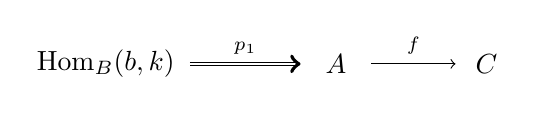
\begin{tikzpicture}[x=1.6em,y=1em]
  \node (a) at (0,0)   {$\HomB(b,k)$};
  \node (b) at (5.2,0) {$A$};
  \node (c) at (8.6,0) {$C$};
  \draw[double,->] (1.9,0) -- node[above]{$\scriptstyle p_{1}$} (4.4,0);
  \draw[->] (6.0,0) -- node[above]{$\scriptstyle f$} (7.9,0);
\end{tikzpicture}
\end{center}
的\trLimit。
对偶的结果把 $f$ 沿 $k$ 的逐点左\trExtension{}在 $b$ 处取的值，表达为%
\trFunctor{} $f$ 沿 $p_{0}\colon\HomB(k,b)\twoheadrightarrow A$ 的限制的%
\trColimit。

我们现在证明：在一个 $(\infty,1)$-\trCategory{}的\trInfinityCosmos{}中，若
一个∞-\trCategory{} $C$ 容有这样的\trLimit，则 $f$ 沿 $k$ 的逐点右%
\trExtension{}存在。对偶的结果把逐点左\trExtension{}的存在性问题约化为某些%
\trColimit{}的存在性问题。

\begin{theorem}[逐点右扩张的存在性]\label{thm:existence-pointwise-right-extensions}
设 $k\colon A\to B$ 是 $(\infty,1)$-\trCategory{}的\trInfinityCosmos{}中的
一个\trFunctor，并设 $C$ 是一个对一切\trElement{} $b\colon 1\to B$ 都容有
$\HomB(b,k)$ 形状的\trLimit{}的∞-\trCategory。那么 $C$ 容有沿 $k$ 的逐点
右扩张
\begin{center}
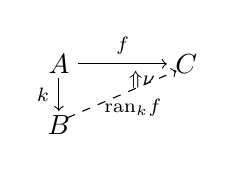
\begin{tikzpicture}[x=1em,y=1em]
  \node at (0,2.2) {$A$};
  \node at (4.6,2.2) {$C$};
  \node at (0,0) {$B$};
  \draw[->] (0.7,2.2) -- node[above]{$\scriptstyle f$} (3.9,2.2);
  \draw[->] (0,1.7) -- node[left]{$\scriptstyle k$} (0,0.5);
  \draw[->,dashed] (0.3,0.25) -- node[below,pos=0.6]{$\scriptstyle\mathrm{ran}_{k}f$} (4.25,1.95);
  \node at (3.0,1.62) {$\scriptstyle\Uparrow\nu$};
\end{tikzpicture}
\end{center}
\end{theorem}

\begin{proof}
考虑从 $A$ 到 $B$ 的模 $\HomB(B,k)$，它由\trFunctor{} $k\colon A\to B$ 协变
表示。\cref{cor:module-equipment-biclosed-cosmos}证明：任何
$(\infty,1)$-\trCategory{}的\trInfinityCosmos{}都容有左 hom 与右 hom，它们
在模的\trVirtualEquipment{}中定义右扩张与右提升。特别地，给定任何\trDiagram{}
$f\colon A\to C$，在模的\trVirtualEquipment{}中存在一个右扩张
\begin{center}
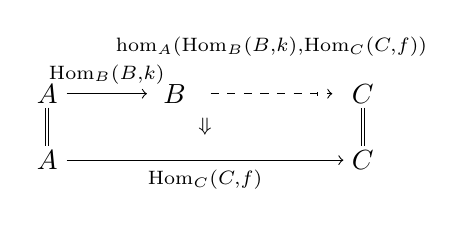
\begin{tikzpicture}[x=1em,y=1em]
  \node at (0,1.2)    {$A$};
  \node at (4.6,1.2)  {$B$};
  \node at (11.4,1.2) {$C$};
  \node at (0,-1.2)   {$A$};
  \node at (11.4,-1.2){$C$};
  \draw[->] (0.7,1.2)  -- node[above]{$\scriptstyle\HomB(B,k)$} (3.6,1.2);
  \draw[->,dashed] (5.9,1.2) -- node[above=10pt]{$\scriptstyle\hom_{A}(\HomB(B,k),\HomC(C,f))$} (10.3,1.2);
  \draw (9.75,1.12) -- (9.75,1.28);
  \draw[->] (0.7,-1.2) -- node[below]{$\scriptstyle\HomC(C,f)$} (10.7,-1.2);
  \draw[double,double distance=0.6pt] (0,0.7)   -- (0,-0.7);
  \draw[double,double distance=0.6pt] (11.4,0.7) -- (11.4,-0.7);
  \node at (5.7,0) {$\scriptstyle\Downarrow$};
\end{tikzpicture}
\end{center}

如今，∞-\trCategory{} $C$ 容有 $f\colon A\to C$ 沿 $k\colon A\to B$ 的逐点
右\trKanExtension，恰当模 $\hom_{A}(\HomB(B,k),\HomC(C,f))$ 被一个\trFunctor{}
$r\colon B\to C$ 协变表示之时。由\cref{cor:pointwise-covariant-representability}，
这条模是协变表示的，当且仅当它沿每个顶点 $b\colon 1\to B$ 的诸\trPullback{}%
是协变表示的，而这又恰当模
$\hom_{A}(\HomB(B,k),\HomC(C,f))\twoheadrightarrow B\times C$ 在 $b$ 之上的%
\trFiber{}拥有一个\trTerminal{}元素之时。

由第 9 章中的\cref{lem:canonical-restriction-cells}，
\trFiber{} $\hom_{A}(\HomB(B,k),\HomC(C,f))(1,b)$ 作为右扩张
\begin{center}
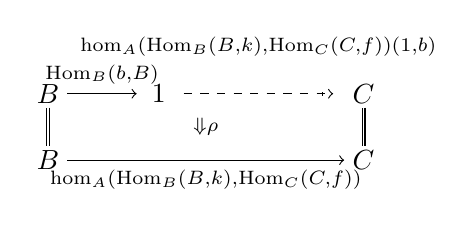
\begin{tikzpicture}[x=1em,y=1em]
  \node at (0,1.2)    {$B$};
  \node at (4.0,1.2)  {$1$};
  \node at (11.4,1.2) {$C$};
  \node at (0,-1.2)   {$B$};
  \node at (11.4,-1.2){$C$};
  \draw[->] (0.7,1.2)  -- node[above]{$\scriptstyle\HomB(b,B)$} (3.2,1.2);
  \draw[->,dashed] (4.9,1.2) -- node[above=10pt]{$\scriptstyle\hom_{A}(\HomB(B,k),\HomC(C,f))(1,b)$} (10.3,1.2);
  \draw (9.9,1.12) -- (9.9,1.28);
  \draw[->] (0.7,-1.2) -- node[below]{$\scriptstyle\hom_{A}(\HomB(B,k),\HomC(C,f))$} (10.7,-1.2);
  \draw[double,double distance=0.6pt] (0,0.7)   -- (0,-0.7);
  \draw[double,double distance=0.6pt] (11.4,0.7) -- (11.4,-0.7);
  \node at (5.7,0) {$\scriptstyle\Downarrow\rho$};
\end{tikzpicture}
\end{center}
而出现。由于 $\HomB(B,k)\otimes\HomB(b,B)\simeq\HomB(b,k)$（第 8 章
中的命题 8.4.7），第 9 章中的\cref{prop:right-extension-associativity}容许
我们把这两个右扩张合并为一个
\begin{center}
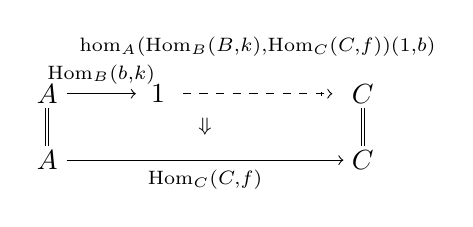
\begin{tikzpicture}[x=1em,y=1em]
  \node at (0,1.2)    {$A$};
  \node at (4.0,1.2)  {$1$};
  \node at (11.4,1.2) {$C$};
  \node at (0,-1.2)   {$A$};
  \node at (11.4,-1.2){$C$};
  \draw[->] (0.7,1.2)  -- node[above]{$\scriptstyle\HomB(b,k)$} (3.2,1.2);
  \draw[->,dashed] (4.9,1.2) -- node[above=10pt]{$\scriptstyle\hom_{A}(\HomB(B,k),\HomC(C,f))(1,b)$} (10.3,1.2);
  \draw (9.9,1.12) -- (9.9,1.28);
  \draw[->] (0.7,-1.2) -- node[below]{$\scriptstyle\HomC(C,f)$} (10.7,-1.2);
  \draw[double,double distance=0.6pt] (0,0.7)   -- (0,-0.7);
  \draw[double,double distance=0.6pt] (11.4,0.7) -- (11.4,-0.7);
  \node at (5.7,0) {$\scriptstyle\Downarrow$};
\end{tikzpicture}
\end{center}

由\trCommaSquare{}的正合性
\begin{center}
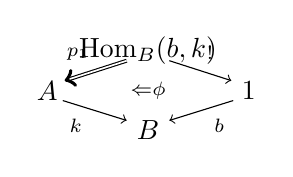
\begin{tikzpicture}[x=1.4em,y=1.2em]
  \node at (0,2.4)    {$\HomB(b,k)$};
  \node at (-2.6,1.2) {$A$};
  \node at (2.6,1.2)  {$1$};
  \node at (0,0)      {$B$};
  \draw[double,->] (-0.55,2.1) -- node[above left,pos=0.45]{$\scriptstyle p_{1}$} (-2.15,1.5);
  \draw[->] (0.55,2.1)  -- node[above right,pos=0.45]{$\scriptstyle !$} (2.15,1.5);
  \draw[->] (-2.2,0.9)  -- node[below left,pos=0.45]{$\scriptstyle k$} (-0.55,0.3);
  \draw[->] (2.2,0.9)   -- node[below right,pos=0.45]{$\scriptstyle b$} (0.55,0.3);
  \node at (0,1.2) {$\scriptstyle\Leftarrow\phi$};
\end{tikzpicture}
\end{center}
我们还有一个复合关系
$\HomA(p_{1},A)\otimes\HomOne(1,!)\simeq\HomB(b,k)$。由第 9 章中的%
\cref{lem:canonical-restriction-cells}，存在一个右扩张图
\begin{center}
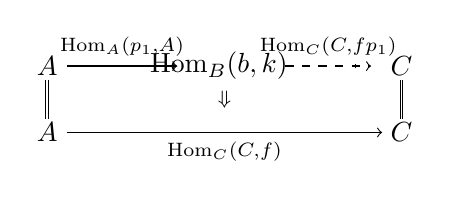
\begin{tikzpicture}[x=1em,y=1em]
  \node at (0,1.2)    {$A$};
  \node at (6.2,1.2)  {$\HomB(b,k)$};
  \node at (12.8,1.2) {$C$};
  \node at (0,-1.2)   {$A$};
  \node at (12.8,-1.2){$C$};
  \draw[->] (0.7,1.2)  -- node[above]{$\scriptstyle\HomA(p_{1},A)$} (4.7,1.2);
  \draw[->,dashed] (8.6,1.2) -- node[above]{$\scriptstyle\HomC(C,fp_{1})$} (11.7,1.2);
  \draw (11.15,1.12) -- (11.15,1.28);
  \draw[->] (0.7,-1.2) -- node[below]{$\scriptstyle\HomC(C,f)$} (12.1,-1.2);
  \draw[double,double distance=0.6pt] (0,0.7)   -- (0,-0.7);
  \draw[double,double distance=0.6pt] (12.8,0.7) -- (12.8,-0.7);
  \node at (6.4,0) {$\scriptstyle\Downarrow$};
\end{tikzpicture}
\end{center}
由于 $\HomC(C,f)$ 沿 $\HomA(p_{1},A)\otimes\HomOne(1,!)$ 容有一个右
扩张，由第 9 章中的\cref{prop:right-extension-associativity}，
$\HomC(C,fp_{1})$ 沿 $\HomOne(1,!)$ 的右扩张存在，且由下图给出：
\begin{center}
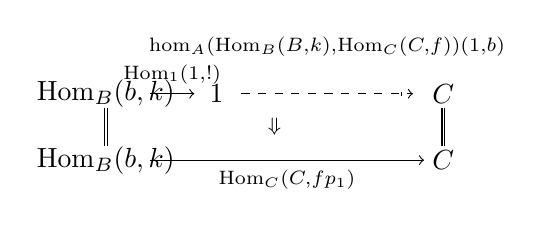
\begin{tikzpicture}[x=1em,y=1em]
  \node at (0,1.2)    {$\HomB(b,k)$};
  \node at (4.0,1.2)  {$1$};
  \node at (12.2,1.2) {$C$};
  \node at (0,-1.2)   {$\HomB(b,k)$};
  \node at (12.2,-1.2){$C$};
  \draw[->] (1.6,1.2)  -- node[above]{$\scriptstyle\HomOne(1,!)$} (3.2,1.2);
  \draw[->,dashed] (4.9,1.2) -- node[above=10pt]{$\scriptstyle\hom_{A}(\HomB(B,k),\HomC(C,f))(1,b)$} (11.1,1.2);
  \draw (10.7,1.12) -- (10.7,1.28);
  \draw[->] (1.6,-1.2) -- node[below]{$\scriptstyle\HomC(C,fp_{1})$} (11.5,-1.2);
  \draw[double,double distance=0.6pt] (0,0.7)   -- (0,-0.7);
  \draw[double,double distance=0.6pt] (12.2,0.7) -- (12.2,-0.7);
  \node at (6.1,0) {$\scriptstyle\Downarrow$};
\end{tikzpicture}
\end{center}
总结起来：模 $\hom_{A}(\HomB(B,k),\HomC(C,f))$ 在\trElement{}
$b\colon 1\to B$ 之上的\trFiber，就是由 $\HomC(C,fp_{1})$ 沿
$\HomOne(1,!)$ 的右扩张所定义的那条模。于是我们看到：若这条模由一个%
\trElement{} $c\colon 1\to C$ 表示，则该\trElement{}定义\trDiagram
\begin{center}
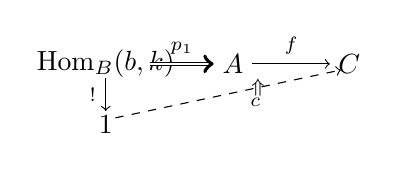
\begin{tikzpicture}[x=1em,y=1em]
  \node at (0,2.2)    {$\HomB(b,k)$};
  \node at (4.6,2.2)  {$A$};
  \node at (8.8,2.2)  {$C$};
  \node at (0,0)      {$1$};
  \draw[double,->] (1.6,2.2) -- node[above]{$\scriptstyle p_{1}$} (3.9,2.2);
  \draw[->] (5.3,2.2) -- node[above]{$\scriptstyle f$} (8.1,2.2);
  \draw[->] (0,1.7) -- node[left]{$\scriptstyle !$} (0,0.5);
  \draw[->,dashed] (0.35,0.25) -- node[below,pos=0.62]{$\scriptstyle c$} (8.5,1.98);
  \node at (5.5,1.35) {$\scriptstyle\Uparrow$};
\end{tikzpicture}
\end{center}
的一个逐点右\trExtension。由第 9 章中的\cref{def:limit-colimit-diagrams}，
它恰在\trDiagram{} $fp_{1}\colon\HomB(b,k)\twoheadrightarrow C$ 在 $C$ 中%
拥有\trLimit{}时存在。既然我们已经假设这个\trLimit{}在 $C$ 中存在，$f$ 沿 $k$ 的逐点右%
\trExtension{}便随之存在，如所宣称。
\end{proof}

由第 10 章中的观察 10.3.4 回忆起：$(\infty,1)$-\trCategory{}的%
\trInfinityCosmos{}容有弱定义的指数。

\begin{corollary}\label{cor:pointwise-right-extension-right-adjoint}
设 $k\colon A\to B$ 是 $(\infty,1)$-\trCategory{}的\trInfinityCosmos{}中的
一个\trFunctor，并设 $C$ 是一个对一切\trElement{} $b\colon 1\to B$ 都容有
$\HomB(b,k)$ 形状的\trLimit{}的∞-\trCategory。那么，逐点右扩张定义限制%
\trFunctor{}的一个右伴随：
\begin{center}
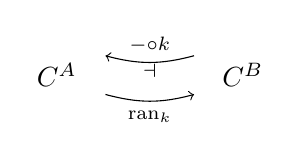
\begin{tikzpicture}[x=1.6em,y=1.4em]
  \node (a) at (0,0)   {$C^{A}$};
  \node (b) at (4.2,0) {$C^{B}$};
  \draw[->] (3.1,0.5) to[bend left=15] node[above,pos=0.5]{$\scriptstyle-\circ k$} (1.1,0.5);
  \node at (2.1,0.12) {$\scriptstyle\dashv$};
  \draw[->] (1.1,-0.5) to[bend right=15] node[below,pos=0.5]{$\scriptstyle\mathrm{ran}_{k}$} (3.1,-0.5);
\end{tikzpicture}
\end{center}
\end{corollary}

\begin{proof}
由第 2 章中的引理 2.3.7，要定义限制的一个右伴随，只需定义恒同穿过\trFunctor{}
$-\circ k\colon C^{B}\to C^{A}$ 的一个\trAbsoluteRightLifting。由%
\cref{prop:absolute-right-lifting-pointwise}，要做到这一点，只需对 $C^{A}$ 的
一切\trElement{} $f\colon 1\to C^{A}$ 定义\trAbsoluteRightLifting{}图表
\begin{center}
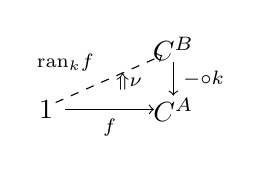
\begin{tikzpicture}[x=1em,y=1em]
  \node at (0,0)     {$1$};
  \node at (4.6,2.2) {$C^{B}$};
  \node at (4.6,0)   {$C^{A}$};
  \draw[->,dashed] (0.35,0.25) -- node[above left,pos=0.45]{$\scriptstyle\mathrm{ran}_{k}f$} (4.2,1.95);
  \draw[->] (4.6,1.7) -- node[right]{$\scriptstyle-\circ k$} (4.6,0.5);
  \draw[->] (0.7,0) -- node[below]{$\scriptstyle f$} (3.9,0);
  \node at (3.0,1.0) {$\scriptstyle\Uparrow\nu$};
\end{tikzpicture}
\end{center}
正如我们的记号所暗示的，我们将论证：\cref{thm:existence-pointwise-right-extensions}
的逐点右扩张 $\nu\colon\mathrm{ran}_{k}f\circ k\Rightarrow f$ 经由第 10 章中的
观察 10.3.4 的\trEquivalence{} $\mathrm{hFun}(X,C^{A})\simeq\mathrm{hFun}(X\times A,C)$
转置，而定义一个\trAbsoluteRightLifting{}图表。

刻画\trAbsoluteRightLifting{}图表的\trUniversalProperty
\begin{center}
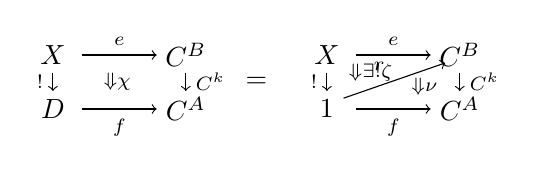
\begin{tikzpicture}[x=1.5em,y=1.3em]
  \node (x1) at (0,1.5)  {$X$};
  \node (cb1) at (3.2,1.5){$C^{B}$};
  \node (d1) at (0,0)    {$D$};
  \node (ca1) at (3.2,0) {$C^{A}$};
  \draw[->] (0.7,1.5) -- node[above]{$\scriptstyle e$} (2.5,1.5);
  \draw[->] (0,1.0) -- node[left]{$\scriptstyle !$} (0,0.5);
  \draw[->] (3.2,1.0) -- node[right]{$\scriptstyle C^{k}$} (3.2,0.5);
  \draw[->] (0.7,0) -- node[below]{$\scriptstyle f$} (2.5,0);
  \node at (1.55,0.75) {$\scriptstyle\Downarrow\chi$};
  \node at (4.9,0.75) {$=$};
  \begin{scope}[shift={(6.6,0)}]
    \node (x2) at (0,1.5)  {$X$};
    \node (cb2) at (3.2,1.5){$C^{B}$};
    \node (o2) at (0,0)    {$1$};
    \node (ca2) at (3.2,0) {$C^{A}$};
    \draw[->] (0.7,1.5) -- node[above]{$\scriptstyle e$} (2.5,1.5);
    \draw[->] (0,1.0) -- node[left]{$\scriptstyle !$} (0,0.5);
    \draw[->] (3.2,1.0) -- node[right]{$\scriptstyle C^{k}$} (3.2,0.5);
    \draw[->] (0.7,0) -- node[below]{$\scriptstyle f$} (2.5,0);
    \draw[->] (0.4,0.3) -- node[above left,pos=0.5]{$\scriptstyle r$} (2.85,1.28);
    \node at (1.05,1.0) {$\scriptstyle\Downarrow\exists!\zeta$};
    \node at (2.35,0.62) {$\scriptstyle\Downarrow\nu$};
  \end{scope}
\end{tikzpicture}
\end{center}
其中我们已记 $r\coloneqq\mathrm{ran}_{k}f$——转置为
\begin{center}
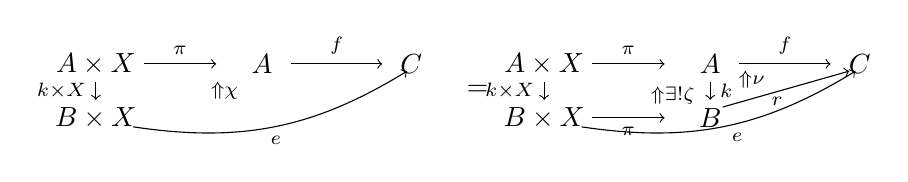
\begin{tikzpicture}[x=1.5em,y=1.3em]
  \node (ax1) at (0,1.5)  {$A\times X$};
  \node (a1) at (4.0,1.5) {$A$};
  \node (c1) at (7.6,1.5) {$C$};
  \node (bx1) at (0,0)    {$B\times X$};
  \draw[->] (1.15,1.5) -- node[above]{$\scriptstyle\pi$} (2.9,1.5);
  \draw[->] (4.7,1.5) -- node[above]{$\scriptstyle f$} (6.9,1.5);
  \draw[->] (0,1.0) -- node[left]{$\scriptstyle k\times X$} (0,0.5);
  \draw[->] (0.9,-0.25) to[bend right=20] node[below,pos=0.5]{$\scriptstyle e$} (7.5,1.3);
  \node at (3.1,0.75) {$\scriptstyle\Uparrow\chi$};
  \node at (9.2,0.75) {$=$};
  \begin{scope}[shift={(10.8,0)}]
    \node (ax2) at (0,1.5)  {$A\times X$};
    \node (a2) at (4.0,1.5) {$A$};
    \node (c2) at (7.6,1.5) {$C$};
    \node (bx2) at (0,0)    {$B\times X$};
    \node (b2) at (4.0,0)   {$B$};
    \draw[->] (1.15,1.5) -- node[above]{$\scriptstyle\pi$} (2.9,1.5);
    \draw[->] (4.7,1.5) -- node[above]{$\scriptstyle f$} (6.9,1.5);
    \draw[->] (0,1.0) -- node[left]{$\scriptstyle k\times X$} (0,0.5);
    \draw[->] (4.0,1.0) -- node[right]{$\scriptstyle k$} (4.0,0.5);
    \draw[->] (1.15,0) -- node[below]{$\scriptstyle\pi$} (2.9,0);
    \node at (0.62,0.95) {$\scriptstyle\lrcorner$};
    \draw[->] (4.3,0.3) -- node[below left,pos=0.55]{$\scriptstyle r$} (7.35,1.3);
    \draw[->] (0.9,-0.25) to[bend right=20] node[below,pos=0.55]{$\scriptstyle e$} (7.5,1.3);
    \node at (3.1,0.62) {$\scriptstyle\Uparrow\exists!\zeta$};
    \node at (5.0,1.05) {$\scriptstyle\Uparrow\nu$};
  \end{scope}
\end{tikzpicture}
\end{center}
第 9 章中的\cref{lem:trivial-exact-squares}证明该\trPullback{}方块是正合的。
现在，若 $\nu$ 是一个逐点右扩张，则由第 9 章中的%
\cref{cor:pasting-pointwise-right-extension}，$\nu\cdot\pi$ 亦然。这个右扩张
图转置后的\trUniversalProperty{}证明：$\nu$ 定义一个\trAbsoluteRightLifting。
\end{proof}

刚才给出的论证还显示了更多的东西。由第 9 章中的%
\cref{cor:pasting-pointwise-right-extension}，逐点右扩张 $\nu$ 与一个%
\trExactSquare{} $\phi$ 的粘贴复合给出另一个逐点右扩张，如下左图所示；而我
们刚刚证明过，它转置而定义一个\trAbsoluteRightLifting{}图表，如下右图所示：
\begin{center}
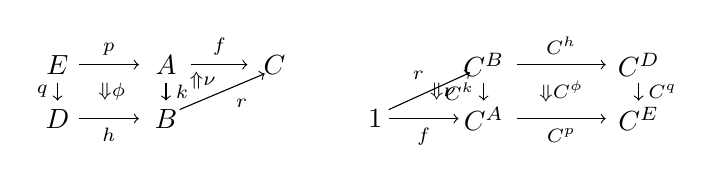
\begin{tikzpicture}[x=1.4em,y=1.3em]
  \node (e1) at (0,1.5) {$E$};
  \node (a1) at (2.8,1.5){$A$};
  \node (c1) at (5.6,1.5){$C$};
  \node (d1) at (0,0)   {$D$};
  \node (b1) at (2.8,0) {$B$};
  \draw[->] (0.55,1.5) -- node[above]{$\scriptstyle p$} (2.1,1.5);
  \draw[->] (3.45,1.5) -- node[above]{$\scriptstyle f$} (4.9,1.5);
  \draw[->] (0,1.0) -- node[left]{$\scriptstyle q$} (0,0.5);
  \draw[->] (2.8,1.0) -- node[right]{$\scriptstyle k$} (2.8,0.5);
  \draw[->] (0.55,0) -- node[below]{$\scriptstyle h$} (2.1,0);
  \draw[->] (3.15,0.25) -- node[below right,pos=0.55]{$\scriptstyle r$} (5.35,1.25);
  \node at (1.4,0.75) {$\scriptstyle\Downarrow\phi$};
  \node at (3.75,1.05) {$\scriptstyle\Uparrow\nu$};
  \node at (7.8,0.75) {$\leftrightsquigarrow$};
  \begin{scope}[shift={(9.6,0)}]
    \node (cb) at (1.4,1.5) {$C^{B}$};
    \node (cd) at (5.4,1.5) {$C^{D}$};
    \node (o)  at (-1.4,0)  {$1$};
    \node (ca) at (1.4,0)   {$C^{A}$};
    \node (ce) at (5.4,0)   {$C^{E}$};
    \draw[->] (2.25,1.5) -- node[above]{$\scriptstyle C^{h}$} (4.55,1.5);
    \draw[->] (1.4,1.0) -- node[left]{$\scriptstyle C^{k}$} (1.4,0.5);
    \draw[->] (5.4,1.0) -- node[right]{$\scriptstyle C^{q}$} (5.4,0.5);
    \draw[->] (2.25,0) -- node[below]{$\scriptstyle C^{p}$} (4.55,0);
    \draw[->] (-1.05,0.25) -- node[above left,pos=0.55]{$\scriptstyle r$} (1.05,1.28);
    \draw[->] (-1.05,0) -- node[below]{$\scriptstyle f$} (0.75,0);
    \node at (0.35,0.75) {$\scriptstyle\Downarrow\nu$};
    \node at (3.4,0.75) {$\scriptstyle\Downarrow C^{\phi}$};
  \end{scope}
\end{tikzpicture}
\end{center}
于是，由转置逐点右扩张图而定义的\trAbsoluteRightLifting{}图表，对与指数化的\trExactSquare{}%
作粘贴保持稳定。特别地，若 $C$ 容有沿 $k\colon A\to B$ 的逐点右扩张，则对
任何\trExactSquare{} $\phi$，我们都有一个\trAbsoluteRightLifting{}图表
\begin{center}
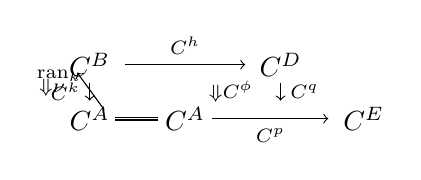
\begin{tikzpicture}[x=1.5em,y=1.3em]
  \node (cb) at (1.8,1.5) {$C^{B}$};
  \node (cd) at (6.4,1.5) {$C^{D}$};
  \node (ca) at (1.8,0)   {$C^{A}$};
  \node (ca2) at (4.1,0)  {$C^{A}$};
  \node (ce) at (8.4,0)   {$C^{E}$};
  \draw[->] (2.65,1.5) -- node[above]{$\scriptstyle C^{h}$} (5.55,1.5);
  \draw[->] (1.8,1.0) -- node[left]{$\scriptstyle C^{k}$} (1.8,0.5);
  \draw[->] (6.4,1.0) -- node[right]{$\scriptstyle C^{q}$} (6.4,0.5);
  \draw[->] (4.75,0) -- node[below]{$\scriptstyle C^{p}$} (7.55,0);
  \draw[double,double distance=0.6pt] (2.4,0) -- (3.45,0);
  \draw[->] (2.15,0.25) -- node[above left,pos=0.5]{$\scriptstyle\mathrm{ran}_{k}$} (1.5,1.28);
  \node at (0.9,0.85) {$\scriptstyle\Downarrow\nu$};
  \node at (5.2,0.75) {$\scriptstyle\Downarrow C^{\phi}$};
\end{tikzpicture}
\end{center}
因为由\cref{prop:absolute-right-lifting-pointwise}，这个\trAbsoluteRightLifting{}图表的%
\trUniversalProperty{}可以在诸\trElement{} $f\colon 1\to C^{A}$ 处逐点检验。
利用这一点，我们可以如下建立一个 derivator 式的「Beck--Chevalley」结果：

\begin{lemma}[Beck--Chevalley]\label{lem:beck-chevalley-mates}
对 $(\infty,1)$-\trCategory{}的\trInfinityCosmos{}中任何\trExactSquare
\begin{center}
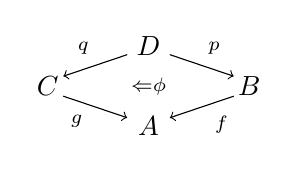
\begin{tikzpicture}[x=1.4em,y=1.2em]
  \node at (0,2.4)  {$D$};
  \node at (-2.6,1.2){$C$};
  \node at (2.6,1.2) {$B$};
  \node at (0,0)    {$A$};
  \draw[->] (-0.55,2.15) -- node[above left,pos=0.45]{$\scriptstyle q$} (-2.2,1.5);
  \draw[->] (0.55,2.15)  -- node[above right,pos=0.45]{$\scriptstyle p$} (2.2,1.5);
  \draw[->] (-2.2,0.9) -- node[below left,pos=0.45]{$\scriptstyle g$} (-0.55,0.25);
  \draw[->] (2.2,0.9)  -- node[below right,pos=0.45]{$\scriptstyle f$} (0.55,0.25);
  \node at (0,1.2) {$\scriptstyle\Leftarrow\phi$};
\end{tikzpicture}
\end{center}
与任何∞-\trCategory{} $E$，受诱导\trNaturalTransformation{} $\phi^{*}$ 的两
个对应 $\phi^{!}$ 与 $\phi_{!}$ 都是\trIsomorphism，只要这些逐点右扩张与左
扩张存在：
\begin{center}
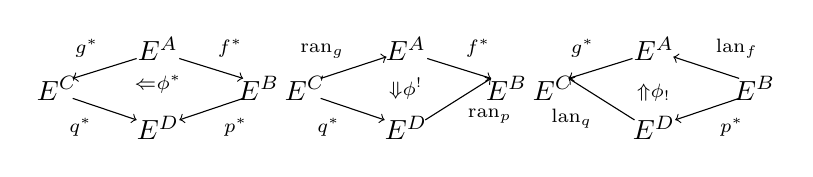
\begin{tikzpicture}[x=1.4em,y=1.2em]
  \node at (0,2.4)    {$E^{A}$};
  \node at (-2.6,1.2) {$E^{C}$};
  \node at (2.6,1.2)  {$E^{B}$};
  \node at (0,0)      {$E^{D}$};
  \draw[->] (-0.55,2.1) -- node[above left,pos=0.45]{$\scriptstyle g^{*}$} (-2.2,1.5);
  \draw[->] (0.55,2.1)  -- node[above right,pos=0.45]{$\scriptstyle f^{*}$} (2.2,1.5);
  \draw[->] (-2.2,0.9)  -- node[below left,pos=0.45]{$\scriptstyle q^{*}$} (-0.55,0.25);
  \draw[->] (2.2,0.9)   -- node[below right,pos=0.45]{$\scriptstyle p^{*}$} (0.55,0.25);
  \node at (0,1.32) {$\scriptstyle\Leftarrow\phi^{*}$};
  \begin{scope}[shift={(6.4,0)}]
    \node at (0,2.4)    {$E^{A}$};
    \node at (-2.6,1.2) {$E^{C}$};
    \node at (2.6,1.2)  {$E^{B}$};
    \node at (0,0)      {$E^{D}$};
    \draw[->] (-2.2,1.5) -- node[above left,pos=0.5]{$\scriptstyle\mathrm{ran}_{g}$} (-0.5,2.15);
    \draw[->] (0.55,2.1) -- node[above right,pos=0.45]{$\scriptstyle f^{*}$} (2.2,1.5);
    \draw[->] (-2.2,0.9) -- node[below left,pos=0.45]{$\scriptstyle q^{*}$} (-0.55,0.25);
    \draw[->] (0.5,0.25) -- node[below right,pos=0.5]{$\scriptstyle\mathrm{ran}_{p}$} (2.2,1.5);
    \node at (0,1.2) {$\scriptstyle\Downarrow\phi^{!}$};
  \end{scope}
  \begin{scope}[shift={(12.8,0)}]
    \node at (0,2.4)    {$E^{A}$};
    \node at (-2.6,1.2) {$E^{C}$};
    \node at (2.6,1.2)  {$E^{B}$};
    \node at (0,0)      {$E^{D}$};
    \draw[->] (-0.55,2.1) -- node[above left,pos=0.45]{$\scriptstyle g^{*}$} (-2.2,1.5);
    \draw[->] (2.2,1.5)  -- node[above right,pos=0.5]{$\scriptstyle\mathrm{lan}_{f}$} (0.5,2.15);
    \draw[->] (-0.5,0.25) -- node[below left,pos=0.5]{$\scriptstyle\mathrm{lan}_{q}$} (-2.2,1.5);
    \draw[->] (2.2,0.9)  -- node[below right,pos=0.45]{$\scriptstyle p^{*}$} (0.55,0.25);
    \node at (0,1.08) {$\scriptstyle\Uparrow\phi_{!}$};
  \end{scope}
\end{tikzpicture}
\end{center}
\end{lemma}

\begin{proof}
由\cref{cor:pointwise-right-extension-right-adjoint}，诸逐点右扩张装配成伴随%
\trFunctor{} $\mathrm{ran}_{g}$ 与 $\mathrm{ran}_{p}$，它们定义\trAbsoluteRightLifting{}图表
\begin{center}
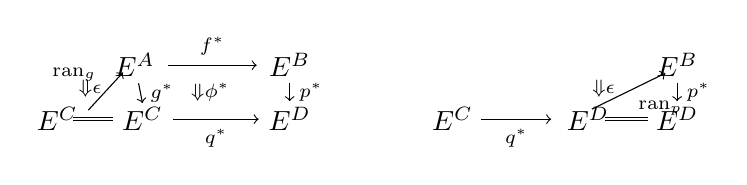
\begin{tikzpicture}[x=1.4em,y=1.3em]
  \node (ea1) at (1.4,1.5)  {$E^{A}$};
  \node (eb1) at (5.4,1.5)  {$E^{B}$};
  \node (ecB2) at (1.6,0)   {$E^{C}$};
  \node (ec0) at (-0.6,0)   {$E^{C}$};
  \node (ed1) at (5.4,0)    {$E^{D}$};
  \draw[->] (2.25,1.5) -- node[above]{$\scriptstyle f^{*}$} (4.55,1.5);
  \draw[->] (1.5,1.0) -- node[right]{$\scriptstyle g^{*}$} (1.6,0.45);
  \draw[->] (5.4,1.0) -- node[right]{$\scriptstyle p^{*}$} (5.4,0.5);
  \draw[double,double distance=0.6pt] (-0.2,0) -- (0.85,0);
  \draw[->] (2.4,0) -- node[below]{$\scriptstyle q^{*}$} (4.6,0);
  \draw[->] (0.2,0.25) -- node[above left,pos=0.5]{$\scriptstyle\mathrm{ran}_{g}$} (1.1,1.3);
  \node at (0.25,0.85) {$\scriptstyle\Downarrow\epsilon$};
  \node at (3.35,0.75) {$\scriptstyle\Downarrow\phi^{*}$};
  \begin{scope}[shift={(10.2,0)}]
    \node (eb2) at (5.2,1.5) {$E^{B}$};
    \node (ec2) at (-0.6,0)  {$E^{C}$};
    \node (ed2) at (2.9,0)   {$E^{D}$};
    \node (ed2b) at (5.2,0)  {$E^{D}$};
    \draw[->] (0.15,0) -- node[below]{$\scriptstyle q^{*}$} (1.95,0);
    \draw[double,double distance=0.6pt] (3.35,0) -- (4.45,0);
    \draw[->] (5.2,1.0) -- node[right]{$\scriptstyle p^{*}$} (5.2,0.5);
    \draw[->] (3.0,0.28) -- node[below right,pos=0.5]{$\scriptstyle\mathrm{ran}_{p}$} (4.9,1.28);
    \node at (3.3,0.85) {$\scriptstyle\Downarrow\epsilon$};
  \end{scope}
\end{tikzpicture}
\end{center}
此外，$\phi^{*}$ 的对应 $\phi^{!}$ 定义左图穿过右图的一个因子分解：
\begin{center}
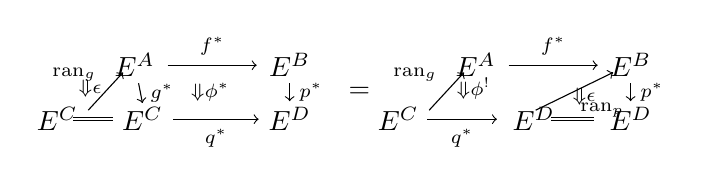
\begin{tikzpicture}[x=1.4em,y=1.3em]
  \node (ea1) at (1.4,1.5)  {$E^{A}$};
  \node (eb1) at (5.4,1.5)  {$E^{B}$};
  \node (ecB2) at (1.6,0)   {$E^{C}$};
  \node (ec0) at (-0.6,0)   {$E^{C}$};
  \node (ed1) at (5.4,0)    {$E^{D}$};
  \draw[->] (2.25,1.5) -- node[above]{$\scriptstyle f^{*}$} (4.55,1.5);
  \draw[->] (1.5,1.0) -- node[right]{$\scriptstyle g^{*}$} (1.6,0.45);
  \draw[->] (5.4,1.0) -- node[right]{$\scriptstyle p^{*}$} (5.4,0.5);
  \draw[double,double distance=0.6pt] (-0.2,0) -- (0.85,0);
  \draw[->] (2.4,0) -- node[below]{$\scriptstyle q^{*}$} (4.6,0);
  \draw[->] (0.2,0.25) -- node[above left,pos=0.5]{$\scriptstyle\mathrm{ran}_{g}$} (1.1,1.3);
  \node at (0.25,0.85) {$\scriptstyle\Downarrow\epsilon$};
  \node at (3.35,0.75) {$\scriptstyle\Downarrow\phi^{*}$};
  \node at (7.2,0.75) {$=$};
  \begin{scope}[shift={(8.8,0)}]
    \node (ea2) at (1.4,1.5)  {$E^{A}$};
    \node (eb2) at (5.4,1.5)  {$E^{B}$};
    \node (ec2) at (-0.6,0)   {$E^{C}$};
    \node (ed2) at (2.9,0)    {$E^{D}$};
    \node (ed2b) at (5.4,0)   {$E^{D}$};
    \draw[->] (2.25,1.5) -- node[above]{$\scriptstyle f^{*}$} (4.55,1.5);
    \draw[->] (5.4,1.0) -- node[right]{$\scriptstyle p^{*}$} (5.4,0.5);
    \draw[->] (0.15,0) -- node[below]{$\scriptstyle q^{*}$} (1.95,0);
    \draw[double,double distance=0.6pt] (3.35,0) -- (4.45,0);
    \draw[->] (0.2,0.25) -- node[above left,pos=0.5]{$\scriptstyle\mathrm{ran}_{g}$} (1.1,1.3);
    \draw[->] (2.95,0.25) -- node[below right,pos=0.45]{$\scriptstyle\mathrm{ran}_{p}$} (4.95,1.3);
    \node at (1.35,0.85) {$\scriptstyle\Downarrow\phi^{!}$};
    \node at (4.2,0.62) {$\scriptstyle\Downarrow\epsilon$};
  \end{scope}
\end{tikzpicture}
\end{center}
直接由 $q^{*}$ 穿过 $p^{*}$ 的\trAbsoluteRightLifting{}的\trUniversalProperty，我们得到
$\phi^{!}$ 是一个\trIsomorphism。$\phi_{!}$ 的证明类似，利用由定义
$\mathrm{lan}_{f}$ 与 $\mathrm{lan}_{q}$ 的逐点左扩张所产生的\trAbsoluteLeftLifting{}图表。
\end{proof}

\subsection*{练习}

\begin{exercise}\label{ex:nonexponentiable-d1}
从单纯集的如下\trPullback{}图
\begin{center}
\begin{tikzpicture}[x=1.6em,y=1.4em]
  \node (a) at (0,1.5)   {$1+1$};
  \node (b) at (4.2,1.5) {$\Lambda^{1}[2]$};
  \node (c) at (0,0)     {$2$};
  \node (d) at (4.2,0)   {$3$};
  \draw[->] (0.9,1.5) -- (3.1,1.5);
  \draw[right hook->] (0,1.0) -- (0,0.5);
  \draw[right hook->] (4.2,1.0) -- (4.2,0.5);
  \draw[->] (0.9,0) -- node[below]{$\scriptstyle d^{1}$} (3.3,0);
  \node at (0.72,0.98) {$\scriptstyle\lrcorner$};
\end{tikzpicture}
\end{center}
推出：\trFunctor{} $d^{1}\colon 2\to 3$ 不可指数化。
\end{exercise}

\begin{exercise}\label{ex:module-cell-right-extension}
设 $A\xrightarrow{E}B$、$A\xrightarrow{G}C$ 与 $B\xrightarrow{R}C$ 是一些模，
并对其配备一个自然\trEquivalence{}
$\Fun_{A\times C}(E\times_{B}F,G)\simeq\Fun_{B\times C}(F,R)$——对一切从 $B$
到 $C$ 的双侧纤维化 $F$。从这个自然\trEquivalence{}中提取一支二元\trCell{}
$\nu\colon E\otimes R\Rightarrow G$，并证明 $\nu$ 展示 $R$ 为 $G$ 沿
$E$ 的一个右扩张。
\end{exercise}

\begin{exercise}\label{ex:model-independent-lemma-12-3-7}
把\cref{lem:pushforward-image-pullback}改编成一个适用于任何
$(\infty,1)$-\trCategory{}的\trInfinityCosmos{}的模型无关陈述，然后证明这个
结果。再用它改编\cref{thm:module-equipment-biclosed}的证明，以直接论证一个
$(\infty,1)$-\trCategory{}的\trInfinityCosmos{}拥有一切左 hom 与右 hom。
\end{exercise}








